% ---------------------------------------------------- %
% Budburst 2015 manuscript
% Preamble
% ---------------------------------------------------- %
\documentclass[11pt]{article}
\usepackage{textcomp}
\usepackage{fontenc}
\usepackage{graphicx}
\usepackage{caption} % for figure captions
\usepackage{gensymb} % for \degree
\usepackage{placeins} % for \images
\usepackage[margin=1in]{geometry} % to set margins
\usepackage{setspace}
\usepackage{lineno}
\usepackage{cite}
\usepackage{amssymb} % for math symbols
\usepackage{amsmath} % for aligning equations

\doublespacing
% \renewcommand{\familydefault}{\sfdefault} % for nicer sans serif font
\graphicspath{{images/}}	% Root directory of the figures
\setlength{\parskip}{2 mm}

\usepackage{Sweave}
\begin{document}

\linenumbers
 
  
\flushleft
\textbf{\large{Coordinated responses to changing environmental cues across a community of temperate forest plants}} % another take


Flynn, Wolkovich

\textit{The Arnold Arboretum of Harvard University}
%%%%%%%%%%%%%%%%%%%%%%%%%%%%%%%%%%%%
% Abstract
%%%%%%%%%%%%%%%%%%%%%%%%%%%%%%%%%%%%


\textbf{Accurate predictions of future spring plant phenology for with continued climate change are critical for robust projections of future growing seasons, plant communities and a related suite of critical ecosystem-level properties. Despite tremendous amounts of observational data of plant phenology progress towards prediction has been hindered because the major cues known to drive phenology---chilling temperatures in fall and winter, photoperiod, and spring forcing temperatures---generally co-vary in nature. Further, research to date using controlled environments to separate these factors suggests that the cues are interactive, meaning accurate predictions of plant responses to climate change will be complex and non-linear \cite{Chuine:1999aa}. Recently, however, other research has suggested many species may be dominated by one of the three possible cues \cite{Korner:2010}, with a tradeoff between photoperiod and forcing temperature sensitivities, meaning some species' responses would be simple to predict. To address this debate we present results of a full-factorial experiment manipulating all three cues (spring forcing temperatures, photoperiod, and intensity of winter chilling ) across 28 woody species and two latitudes (42.5\degree N and 46\degree N) in North American temperate forests. In contrast to the predicted tradeoff between photoperiod and temperature cues we find responses to these cues are  largely coordinated across species; namely, species highly sensitive to temperature were also highly sensitive to photoperiod. Bud burst and leaf-out were more sensitive to temperature than to photoperiod. Winter chilling exerts a large role in driving advances in spring phenology, for both bud burst and leaf out stages, yet more intense chilling at 1.5\degree C resulted in less pronounced effects than at 4\degree C. Latitude of origin exerted surprisingly small effects on sensitivity to abiotic factors in driving spring phenology, indicating that local adaptation---at least across 4\degree of latitude---may not necessarily constrain woody plant responses to climate change. Shrub and small tree species were less sensitive to changing temperatures or photoperiod, but consistently earlier in their phenology. These results indicate that under warming conditions, communities could shift to a more canopy-tree dominated system with generally later phenologies, counteracting advances in phenology at the ecosystem scale.}

% I would keep the shrub/tree distinction; just getting rid of traits results here

%%%%%%%%%%%%%%%%%%%%%%%%%%%%%%%%%%%%
%Introduction 
%%%%%%%%%%%%%%%%%%%%%%%%%%%%%%%%%%%%

Woody plant spring phenology drives local ecosystem properties, from the length of the growing season to energy balance between land and atmosphere, and scales up to impact global carbon cycles \cite{Richardson:2009aa}. The crucial role that phenology plays in ecosystem processes, and the wealth of observational data highlighting how rapidly plant and animal phenology are advancing \cite{Menzel:2006} has led to increased interest in better understanding and prediction of how plant phenology will shift with continued climate change.

Decades of study on wild species spring phenology---mainly focused on temperate woody species---show that three major cues drive bud burst and leaf-out: spring temperatures (forcing), length and intensity of winter temperature (chilling), and changing day length (photoperiod). Across studies increasing temperatures in the spring appear to be a dominant factor that controls spring phenology, yet many of these studies have been observational---making it nearly impossible to tease out the generally co-varying effects of longer days and reduced cold temperatures, which generally reduce chilling. In contrast studies from controlled environments (e.g., growth chambers or greenhouses) have highlighted the additional importance of photoperiod and chilling \cite{Heide:1993b,Falusi:1996aa,Foley:2009aa,Ghelardini:2010aa,Caffarra:2011aa}, with longer days and increased chilling leading to more rapid leaf-out \cite{Caffarra:2011ab}. Further, photoperiod and chilling often appear to interact, as long photoperiod enhances cell growth, compensating for a lack of chilling during plants' winter dormacy \cite{Heide:1993b,Myking:1995,Caffarra:2011aa}. To an extent, all three factors---temperature, photoperiod, and chilling may be interchangeable in some species---such that a plant experiencing a mild winter with insufficient chilling can still break bud given sufficiently long photoperiods and warm temperatures \cite{Heide:1993b}. 

% Caffarra & Donnolley 2011: Tilia and Fagus conservative, late successional and photoperiod-cued; Betula and Salix less conservative and forcing-cued

A major challenge to build on this extensive study of how temperature and photoperiod drive spring phenology is understanding---and possibly predicting---how the sensitivity to each cue and their interactions varies across species. Temperate woody species are well known to  have different sets of cues, depending on the species \cite{Lechowicz:1984aa,Korner:2010}---with some species showing stronger spring forcing or photoperiod cues, for example. A possible framework for understanding this variation in cues comes from considering how adaptive pressures may drive temperate plant phenology \cite{Wolkovich:2011aa,Wolkovich:2014ab}. Temperate woody plants should aim to maximize the carbon gain that comes from starting growth early in the season and gaining first access to critical resources such as light, soil nitrogen and water, while at once minimizing the risk of tissue loss to frost in early spring \cite{Korner:2010,Gu:2008aa,Hufkens:2012aa}. Across a community of co-occuring species we may expect a diversity of strategies to address these pressures---allowing each species to persist in the community. 

The ways that species manage such risks, and possible rewards, can vary in both when on average in the spring they begin their growth, and also how flexible they are around that average timing. Related to this, two tradeoffs have been described for spring phenology of woody plants in response to a variable spring environment: tolerance versus avoidance of freezing \cite{Sakai:1987aa}, and opportunistic versus conservative strategies \cite{Korner:2010}. The former describes how early or late in a season a species leafs out---with tolerant species consistently leafing out early each year, while avoidance species would consistently leaf out late---while the latter describes how flexible a species or individual may be in response to unusually early warm-up events, with opportunistic species tending to have phenological cues that yield variable leaf-out times across variable years and conservative species tending to leaf out consistently across variable years. While related, these tradeoffs predict some differences in the characteristic of the cues and related traits of each species and may combine to produce contrasting changes in phenology. 

Importantly, the combinations of these axes can result in non-intuitive responses at the community level. For example, under a relatively stationary long-term climate early tolerant but conservative species would enjoy the advantage of a long growing season. Yet, as that environment becomes nonstationary---as is the case with climate change---such advantages may quickly eroded. In contrast under a warming environment, species that are relatively late in leafing out (avoidance) and flexible (opportunistic) close the gap with those tolerant species in bud burst and leaf out times. Thus, understanding both the rank order of phenology and the sensitivity of species to environmental cues across a whole community is important in understanding how a changing climate will affect community dynamics. % Opportunistic strategies should benefit species in a nonstationary environment, as in a warming world where mild winters are less an unusual occurrence.

% EMW: Can we say somewhere quickly in below paragraph what the predictions are for phenological cues? It seems like tolerant species would have to have cues to be early (low requirements for everything?) and avoidance species need cues to be late .... If phenological cues for tolerant-avoidance has not been discussed much before we should acknowledge that also. 
For the tolerance-avoidance axis, plants may either tolerate risk of spring freezing in two major ways: through phenological cues that allow them to leaf out well after all frost risk has passed (avoidance) or through investing in tissue which can withstand freezing (tolerant). For perennial plants, it has been found that leaf and wood tissues of species which have later phenologies can be more sensitive to frost damage \cite{CaraDonna:2014aa,Vitasse:2014aa,Lechowicz:1984aa}, supporting the notion of a tradeoff between tolerance and avoidance of freezing risk. In contrast, avoidance-strategy plants would be expected to express lower tissue densities, with the shorter growing season being made up for by faster growth rates, less investment in structural elements of tissue, and relatively greater percent nitrogen in leaves. 

The axis of conservative versus opportunistic strategies makes specific predictions for the phenological cues of differing species and may also predict the related traits of species. In opportunistic plant strategies, temperature is the dominant driver of spring phenology, while for species with conservative strategies, photoperiod and chilling would be the major drivers. It has been found for several cases that short-lived, early successional species typically exhibit such opportunistic strategies, and late-successional species are more typically chilling- and photoperiod-controlled in breaking of dormancy \cite{Korner:2010,Caffarra:2011ab,Basler:2012aa}.

% would like to find a citation for changes in traits within early part of growing season, have not found this.
% other timing and traits: earlier phenology, fleshy fruits \cite{Kjell-Bolmgren:2005aa}, even after doing PIC
% For herbaceous species, two axes: early vs late, and fast vs slow growth. Early-fast, late-slow, late-fast all possible \cite{Sun:2011aa}. Early-fast related to short stature and high relative groth rate

Tests of how these two tradeoff axes drive phenology across a co-occurring community of species have not previously been carried out. As the abiotic environment is not the sole contributor to plant performance, considering a suite of co-occurring species together is key for making progress in understanding the role phenology plays in shifts in community composition and ecosystem functioning \cite{Cleland:2007aa}.

To test the interactive effects of the three controlling drivers of spring phenology, temperature, photoperiod, and chilling across latitudes, we carried out a study of 28 woody plants. We assessed both bud burst and leaf-out to account for the potential different sensitives of these phenological stages to abiotic drivers, and analyzed responses across all species to examine the support for how well the tolerance-avoidance and opportunistic-conservative tradeoff axes represent temperature plant spring phenology.

%%%%%%%%%%%%%%%%%%%%%%%%%%%%%%%%%%%%
\section*{Results}
%%%%%%%%%%%%%%%%%%%%%%%%%%%%%%%%%%%%

Major findings
\begin{itemize}
\item{All of the 28 species showed sensitivity to all three of the abiotic drivers.}
\item{The strength of the sensititivty to each driver was coordinated, not showing a trade-off axis}
\item{Species with greater sensitivity were generally later-phenology, canopy trees, rather than early-season, early-successional shrubs.}
\end{itemize}

Forcing temperature, photoperiod, and chilling individually and interactively determined timing of both bud burst and leaf-out. We found photoperiod sensitivity was common and strong across all of the woody plants studies, consistently reducing time to phenological responses for each species, across sites of origin. 

For the 28 species studied, sensitivity to temperature and photoperiod cues for leaf-out times varied substantially, and---in contrast to our hypotheses [that we set up in the intro]---co-varied overall. The coordinated response to warming temperatures and longer photoperiod was consistent with overall pace of phenological events; earlier-leafing out species (namely the shrubs \emph{Spiraea alba}, \emph{Viburnum cassanoides}, and \emph{Vaccinium myrtilloides}) exhibited relatively limited advances to either warming or longer days, while later leafing-out species showed ability to advance their phenology by in response to both warming and longer days. Thus, no trade-off was observed between photoperiod-cued and temperature-cued species, but rather species exhibit coordinated responses to both environmental factors (Fig. 1). Of the other species, \emph{Fagus grandifolia} exhibits relatively limited response to warming but substantial photoperiod sensitivity, while \emph{Rhamnus frangula} shows relatively limited response to photoperiod but substantial warming sensitivity; if only a small subset of species including these two had been included in the study, it might have been concluded that a tradeoff between photoperiod sensitivity and warming sensitivity would exist. 

While both photoperiod and temperature cues were important for driving woody plant phenology, responses to chilling were also substantial. Bud burst day was accelerated most by the chilling treatments. Tables 1 and 2 summarizes hierarchical mixed-effects model analysis of day of bud burst and leaf-out, with negative values indicate earlier day of experiment for each event. Overall the 5\degree C experimental warming resulted in 6.8 days earlier bud burst and 21.9 days earlier leaf out. Such advance was delayed by the each chilling treatment, as indicated by the positive coefficient for the temperature x chilling interactions. Latitude of origin (Site) overall had little direct effect on bud burst or leaf-out, but populations from the northern site tended to exhibit slower bud burst and leaf-out, with a more rapid bud burst and leaf out in response to the chilling treatments (indicated by negative coefficients for site x chilling treatments).

Warming, photoperiod, and chilling individually and interactively acted to drive bud burst and leaf out earlier across species. The strength of the acceleration in bud burst due to both warming and photoperiod were similar, but the acceleration of leaf out due to warming exceeded that of photoperiod for both phenological stages. Surprisingly, site of origin exerted limited effect on either bud burst or leaf out across species. 

\subsection*{Effect of chilling}
Species varied widely in response to chilling treatments, with some exhibiting strong chilling requirements (\emph{Acer saccharum}, \emph{Fagus grandifolia}), while others exhibited little change in phenological advancement under experimentally manipulated chilling. Overall, bud burst and leaf-out advanced by 22.1 or 26.4 days under additional 30 d of vernalization at 4\degree C, and advanced by a reduced amount of 19.7 or 26.1 days under 30 d of vernalization at 1.5\degree C. The reduced chilling effect at the lower temperature chilling is consistent with the Dynamic Model of chilling accumulation. % And also consistent with the Utah model?

Species-specific responses to chilling demonstrate that chilling requirements are not uniform across species, with 
of \emph{Fagus grandifolia} to increasingly strong vernalization varies by latitude of origin and by phenological stage; winter chilling reduced day to bud burst and leaf-out, but more strongly for individuals from the northern site.

While nearly all species showed advances in spring phenology in response to the experimental chilling treatment, as indicated by fewer days to phenological events for the 4\degree C and 1.5\degree C treatments, the majority of species (e.g. \emph{Populus grandidentata}) showed delays in both bud burst and leaf out at the more severe chilling treatment. Of the species exposed to the additional chilling, only \emph{Fagus grandifolia} was consistently advanced by the more severe chilling.

\subsection*{Species-specific responses}

Species traits partly explain variation in warming and photoperiod sensitivities of leaf out. Plants with high nitrogen leaves, as well as high SLA (thinner, less dense) leaves, were significantly later in both bud burst and leaf out. Thus early leaf out species tended to be tougher, less N-dense, and have higher carbon investments than later species. Greater wood density had inconsistent effects as a driver, with higher wood density driving later bud burst but tending to drive earlier leaf out.

Ring-porous species (\emph{Fraxinus sp.}, \emph{Lonicera}, \emph{Myrica}, and \emph{Quercus}; lower values of Pore Anatomy variable) exhibited significantly later bud burst and leaf out compared to diffuse-porous species, in line with previous work on wood anatomy and freezing risk \cite{Sperry:1992}.

Shrubs with low specific leaf area (thick/dense leaves) and high stem density were more likely to leaf out earlier. For trees, with an overall later leaf out pattern, 

Rank order of leaf out and bud burst was stable across warming and photoperiod treatments. Chilling treatments shifted the order, for example \emph{Fagus grandifolia} was the 23-28th species to burst bud with no additional chilling, but advanced to the 10-11th species to burst bud in with additional chilling. Within chilling treatments, the consistency of the rank order was high, with standard deviation of the rank order ranging from 2.05 d (bud burst, no additional chilling) to 0.75 d (leaf out, additional chilling at 4\degree C). Compared to field observations, rank order of leaf out was generally most related in the cool, short-day treatment with no additional chilling (Fig. S10).




%%%%%%%%%%%%%%%%%%%%%%%%%%%%%%%%%%%%
\section*{Discussion}
%%%%%%%%%%%%%%%%%%%%%%%%%%%%%%%%%%%%

Photoperiod sensitivity is common in northeastern woody plants, and greater photoperiod sensitivity is related to, not instead of, temperature sensitivity. Taken together, this result shows that the opportunism-conservatism tradeoff is not supported by the data for this suite of species. The most sensitive species to both cues, namely the species which could advance their phenology in response to both longer days and warmer temperatures, were the later-successional tree species, rather than the shrubs. The trait data indicate partially that the species earliest to leaf out, namely the shrubs and small trees, also had lower SLA and lower leaf \%N, indicating greater investment in tissue structures. These results support the tolerance-avoidance tradeoff, with the early phenology species being tolerant to freezing but relatively less able to advance their phenology in a warming environment. These results also indicate that the later-successional species have potentially the most to gain from a warming world, as they can extend their growing seasons  

While both photoperiod and temperature sensitives were common, chilling sensitivity greatly outweighed both of these factors. It is important to note that the results from the chilling part of this experiment are derived from 11, not 28 species, but the strength of this effect is notable. Strong chilling requirements were detected both for bud burst and leaf out responses, and the most substantial advance in spring phenology came from the more mild chilling treatment, at 4\degree C, with reduced effectiveness of chilling at 1.5\degree C. 

These three factors did show some degree of substituability, meaning for example that a lack of chilling could be made up for by an increase in temperature. These are indicated by the positive two-way interactions; chilling and forcing temperature are more substitutable than chilling and photoperiod, for both bud burst and leaf out.

We found only limited support for the northern populations showing more conservative (photoperiod-cued) strategies in these 28 species was found, with small delays in both phenological events for populations from the more northern site. The latitudinal range studied here is within the range of the phenotypic flexibility of these species. Of these study species, we should not be overly concerned about being photoperiod limited at the more northern sites; given sufficient pace of dispersal, they will be able to track a changing climate.

bud burst is sensitive to the same environmental cues as leaf out, but species show idiosyncratic orderings of their sensitivity to environmental cues at these two phenological stages; leaf out responses can not necessarily be used to back-cast bud burst responses. Bud burst showed a more limited total response to environmental cues, and species were more tightly clustered in those responses.

Surprisingly, the smaller statured, earlier-leafing out shrubs and small trees exhibited reduced sensitivity to all three factors of temperature, photoperiod, and chilling. They are relatively more fixed in their timing of both bud burst and leaf out, perhaps indicating an alternative mechanism for timing of spring phenology in these plants \cite{Pagter:2015}.

Given these results, the future of the northeastern forests may shift towards later-phenology, canopy trees, as these species demonstrated a greater ability to lengthen their growing seasons opportunistically in response to warmer temperatures.
% I think we should be more cautious in stating this. We still don't know *what* controls their leaf out! -- I think we can make some educated guesses here!

% Re the above about shrubs versus trees -- I am just not sure what to think! And it comes back to the models. Our models give each species a fundamental leaf out day -- their intercept. This makes lots of sense to me but biologically I am not sure what to do with it (and if we take it away then the early species become hyper-sensitive, right? - right). I think we need to think on what that intercept means and what we should and shouldn't say given that it's in our models. I think it could be what you suggested, it could also be that they have super weak chilling, it could be that they are sensitive to humidity or something we don't study. But fundamentally I think we need to think harder about that before we push our conclusions too far. 
%%%%%%%%%%%%%%%%%%%%%%%%%%%%%%%%%%%%
\section*{Methods}
%%%%%%%%%%%%%%%%%%%%%%%%%%%%%%%%%%%%
\textbf{Field sampling}

Woody plant cuttings were made in January 2015 for 28 species which occurred in both Harvard Forest (HF, 42.5\degree N, 72.2\degree W) and the Station de Biologie des Laurentides in St-Hippolyte, Quebec (SH, 45.9\degree N, 74.0\degree W). The typical late January temperatures are -3.4 and -22\degree C, respectively; day length between these two sites differs by a maximum of 45 minutes. Weather station data from each field site was obtained for calculations of chilling units. 

Species were chosen based on the dominant forest vegetation at each site, aiming to maximize the number of shared species between the two sites. Of the 28 species, 19 occurred at both sites. Comparing only shared species, the mean days to bud burst and leaf out across all treatments for Harvard Forest and St. Hippolyte was 25.6/36.8 and 24.8/36.1 days, respectively (Table S1). For each species, up to 15 representative healthy, mature individuals with branches accessible by pole pruners from the ground were tagged in late summer and fall 2014. In winter 2015, six individuals were located and 4-16 cuttings taken from each individual, depending on size of the individual and number of treatments to be applied. Cuttings were kept cold and transported back to the Arnold Arboretum in Boston, MA.
%The species chosen represent XXX percent of the basal area in Harvard Forest and St. Hippolyte, respectively.

\textbf{Growth Chamber Study}

Cuttings were placed in growth chambers at the Arnold Arboretum in Erlenmeyer flasks distilled water, with water changed every 7-10 days. The base of cuttings was re-cut at each water change under water to prevent callusing. For 11 of the 28 species, sufficient cuttings were obtained from each individual tree to apply the full set of 12 experimental treatments: 2 temperature (20\degree C / 10\degree C warm vs. 15\degree C / 5\degree C cool) x 2 photoperiod (12 vs. 8 h) x 3 chilling (no additional chilling,  additional 33 d at 4\degree C, or 33 d at 1.5\degree C) treatments. For the remaining 17 species, only sufficient cuttings were obtained to apply the temperature and photoperiod treatments, without the additional chilling levels. The total number of cuttings for a given species thus ranged from 24 to 144, depending on presence at each site and application of the chilling treatment.

Phenology of the cuttings was assessed using a modified BBCH scale \cite{Finn:2007}, with observations on each of the 2,136 cuttings made every 2-3 days for the course of the 82-day experiment, a total of 48 observation days. The phenological stages assessed in the present study are bud burst, defined as beginning of sprouting or bud breaking or shoot emergence (Code 07 in \cite{Finn:2007}) and leaf out, defined as first leaves unfolded (Code 11 in \cite{Finn:2007}). Additional stages up to flowering and stem elongation were also recorded. In total, we made 19,318 phenological observations at the cutting level.

\textbf{Functional trait collection}
In summer 2015, the same individuals previously tagged in the field were revisited as part of an additional study. Six individuals of each species were sampled for several plant functional traits, following standard protocols \cite{Perez-Harguindeguy:2013aa}. In some cases, the individual used in the growth chamber study was missing, in poor condition, or had no remaining branches to sample, and was replaced by a nearby representative individual. For each individual, height and diameter at breast height (DBH) were recorded, and leaf and stem material were sampled from the middle of the canopy or the greatest height reachable with pole pruners. Leaf material was kept cool and moist, and within several hours was scanned for leaf area and weighed fresh. Stem volume was measured using a water-displacement method. Samples were oven dried at 70\degree C and weighed within several days of sampling, and specific leaf area (SLA) were calculated stem density. Leaf tissue was further processed for carbon:nitrogen ratio using an elemental analyzer (Perkin-Elmer Elemental Analyzer) at Harvard Forest. Since in not all cases the same individual used for the growth chamber experiments was the individual sampled for functional traits.

\textbf{Statistical analysis}

For the two phenology responses measured, bud burst and leaf-out, we fit mixed effect hierarchical models using site, warming, photoperiod, and chilling treatments as predictors (fixed effects) and species as a modeled groups (random effects). For each model, two-way interactions for effects of site, warming, and each of the chilling treatments were included. The models were fit using a Markov Chain Monte Carlo sampling approach in the programming language \texttt{Stan} \cite{Carpenter:2016aa}(\texttt{www.mc-stan.org}), accessed via the \textit{rstan} package in R \texttt{www.r-project.org}.

The model was fit using a Baeysian approach with weak priors with five main effects and each of their two-way interactions, which allowed us to calculate the posterior probabilities of the effects for each of the abiotic drivers individually and interactively. We ran four chains simultaneously, with 2 500 burn-in iterations followed by 2 500 sampling iterations, resulting in 10 000 posterior samples for each parameter. The model was fit as follows:

\begin{align*}
y_i \thicksim N(\alpha_{sp[i]} +& \beta_{site_{sp[i]}} + \beta_{temperature_{sp[i]}} + \beta_{photoperiod_{sp[i]}} + \beta_{chilling1_{sp[i]}} + \beta_{chilling2_{sp[i]}}  \\
	+& \beta_{temperature \times photoperiod_{sp[i]}} + \beta_{temperature \times site_{sp[i]}} + \beta_{photoperiod \times site_{sp[i]}} \\
	+& \beta_{temperature \times chilling1_{sp[i]}} + \beta_{temperature \times chilling2_{sp[i]}} \\
	+& \beta_{photoperiod \times chilling1_{sp[i]}} + \beta_{photoperiod \times chilling2_{sp[i]}} \\
	+& \beta_{site \times chilling1_{sp[i]}}  + \beta_{site \times chilling2_{sp[i]}} )
\end{align*}

Each of the 14 $\beta$ coefficients was modeled at the species level, as follows
\begin{align*}
1.& \; \beta_{site_{sp}} \thicksim N(\mu_{site}, \sigma{^2}_{site}) \\
   &... \\
14.& \; \beta_{site \times chilling2_{sp}} \thicksim N(\mu_{site \times chilling2}, \sigma{^2}_{site \times chilling2})
\end{align*}

For the $mu$ and $sigma$ parameters, weakly informative priors were chosen.

\textbf{Phylogenetic methods}

We tested the influenced of phylogenetic relatedness on the relationship between functional traits and sensitivities to warming, photoperiod, and chilling treatment. Sensitivities were extracted as the slopes of the species-level responses of leaf out day to each of the experimental factors; more negative values indicate greater advance in leaf out in response to that factor. Using a phylogenetic tree resolved at the genus level from Phylomatic (\texttt{www.phylodiversity.net}), and the \emph{caper} package in \texttt{R}, we fit phylogenetic generalized linear models between the sensitivities at the species level to the functional traits of stem density, SLA, and percent leaf nitrogen (\%N). In this type of model, the parameter $\lambda$ represents the strength of the phylogenetic symbol, with values close to 1 indicating that closely related species have more similar responses to the abiotic drivers.

%%%%%%%%%%%%%%%%%%%%%%%%%%%%%%%%%%%%
\section*{References Cited}
%%%%%%%%%%%%%%%%%%%%%%%%%%%%%%%%%%%%

\bibliography{danlib}
\bibliographystyle{naturemag}

\end{document}

%%%%%%%%%%%%%%%%%%%%%%%%%%%%%%%%%%%%
\section*{Figures and Tables}
%%%%%%%%%%%%%%%%%%%%%%%%%%%%%%%%%%%%

%\listoftables
%\listoffigures





%%%%%%%%%%% Figures
% 1. Experimental design

% 2. model output
\begin{figure}
\begin{center}
\caption{Modeled effects plots, bud burst and leaf out}
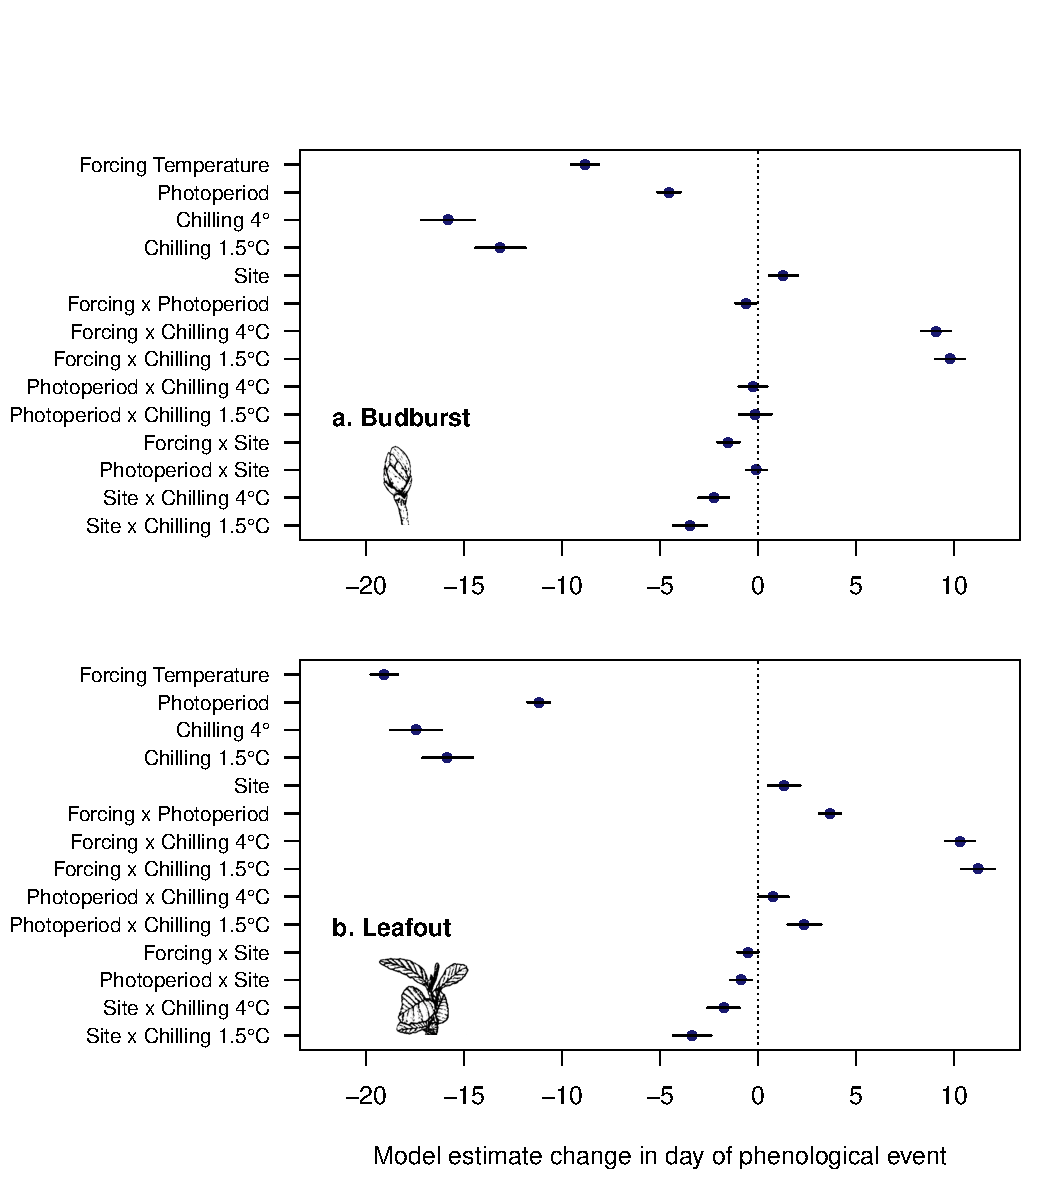
\includegraphics[scale=0.8]{Fig1_bb_lo}
\label{fig2}
\end{center}
\end{figure}

% 3. Temp + Pheno + Chill sensitivity

\begin{figure}
\caption{Sensitivity of bud burst and leaf out to warming, leaf out, and chilling.}
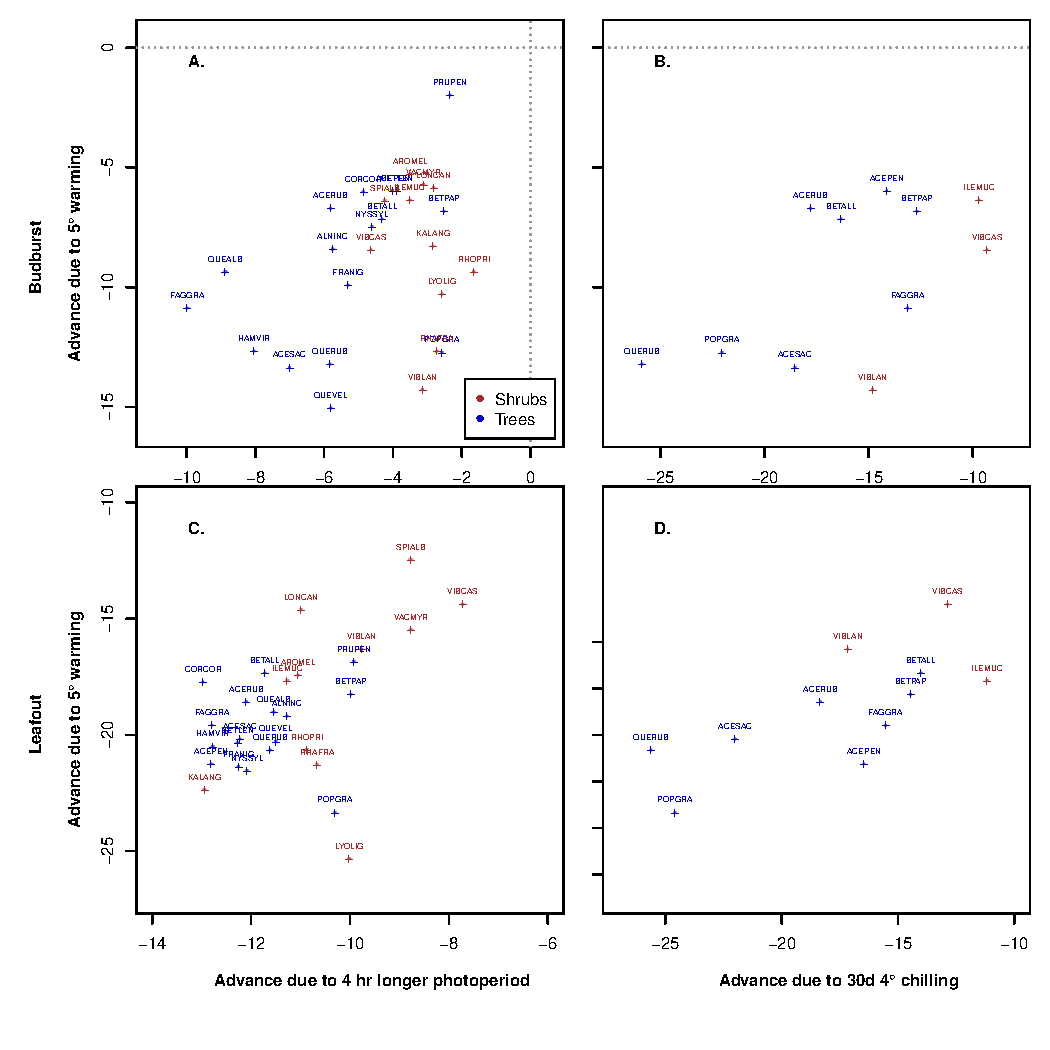
\includegraphics[scale=0.9]{Fig2_4panel}
\label{fig3}
\end{figure}

\end{document}}



%%%%%%%%%%%%%%%%%%%%
%%%%%%% EDITS %%%%%%%%%
%%%%%%%%%%%%%%%%%%%%

%%% From the intro: 

% Traits/strategies
Physiologically, tolerance to freezing is driven by resistance to rupturing of biomembranes, and is related to dehydration stress \cite{Larcher:2005aa}. 

Different phenological stages may be driven by different environmental cues. The period between bud burst and leaf out is critical for leaf development, as this is a period when plants are highly sensitive to damage from late freezing events, with freezing resistance increasing as leaves expand \cite{Sakai:1987aa}.

Drought-tolerance, which can be related to freezing-tolerance in the ability to resist cavitation, has been show to relate to low wood density in a semi-arid forest, with low-wood density species having increased ability to store water in the dry season and ability to flush leaves in the dry season \cite{Lima:2010aa}. Similarly, for temperate deciduous trees, experimental warming has been shown to both increase total growing season length for species which have higher specific leaf area \cite{Xu:2009aa}. Finally, for deciduous trees, traits can exhibit variation in expression over the growing season, with higher leaf tissue density and allocation of nitrogen following cessation of growth in late summer \cite{McKown:2013aa}.

% Community angle
Temporal separation in resource use is an important driver of plant species coexistence \cite{Mason:2013aa} and such temporal separation can drive ecosystem properties such as biomass accumulation \cite{Sapijanskas:2014aa}, thus understanding both the current order of phenology for co-occurring species and propensity to change in future climates is an important goal of plant phenology science.

% Why do cuttings: can manipulate abiotic conditions on same individual, species specific, can detect early events with more precision than larger-scale studies
Knowing species-specific sensitives of temperate plant phenology to chilling and forcing alone can predict regional-scale phenology \cite{Chuine:2000}. Substantial variation exists at the species level in the magnitude of the temporal advance of spring phenology \cite{Primack:2009aa}, such that the presence of species highly sensitive to temperature change can strongly drive community-level phenology \cite{Diez:2012}.

% Latitude
Factors driving spring phenology include chilling temeratures, photoperiod, forcing temperatures, and latitude of origin. Of these factors, the role of latitude in determining spring phenology has largely been investigated in single-species studies across many sites. Given sufficient distance, more pole-ward sites have lower minimum annual temperatures and shorter growing seasons, making accurate timing of spring phenology even more important. Since day length differences from winter to spring are also greater for higher latitudes, populations of northern plants may be expected to rely more on photoperiod as a cue for spring phenology.

For temperate trees, species can be limited at their northern range by inability to develop mature fruit in a given growing season, while limited at their southern range by inability to break dormancy due to insufficient chilling \cite{Chuine:2010}. Thus phenology can drive range limits. Common garden studies have shown that southern-adapted species, when translocated to a more northern location, exhibit later leaf out compared to species adapted to northern sites \cite{Zohner:2014aa}. If species remain relatively fixed in their timing of leaf out, then northward migration of such late-phenology species may act to counteract community-wide advances in phenology under a warming climate. 

% photoperiod
Photoperiod has long been known to be a critical driver of the onset of endodormancy, in combination with cooling temperatures \cite{Foley:2009aa}. However, the role of photoperiod in determining the breaking of dormancy has been debated, with various authors finding that the strength of day length as a driver may depend on phenological stage, species and location \cite{Heide:1993,Falusi:1996aa}. 

In the few experimental studies that have directly manipulated both forcing temperature and photoperiod, photoperiod has been shown to act to moderate advances in phenology due to warming, with reduced advances due to temperature when day length was short \cite{Heide:1993b,Sanz-Perez:2009aa}. 
% look for additional refs showing non-additive effects (replacability)

% Chilling
% points to make: chilling is a strategy to make sure bud burst/leaf out do not occur too early. This can be a supplemental stragety in addition to photoperiod and temperature cues for breaking endodormancy. [notes to myself: endodormancy: short days in fall. Broken by chilling. Ecodormancy: broken by temperature.

In addition to photoperiod, winter chilling requirements also act as a conservative strategy to avoid damage from early spring freezing, allowing woody plants to avoid breaking bud during unusually early warm spells \cite{Ghelardini:2010aa}.

Chilling requirements are known to vary substantially across species, with some needing relatively little winter chilling to initiate bud burst, and others not bursting bud even in long-day, warm environments unless sufficient chilling has taken place \cite{Korner:2010}. 



